%% -----------------------------------------------------
%% Sample NSERC Alliance proposal template
%%
%% - Declare the document as "nserc-alliance",
%%   and specify whether the document is in French or English.
%% - Optionally, you can use the argument "nobullets" to hide all
%%   the instructions under each section title, and leave only
%%   your text.
%% - The pdf14 option can reduce PDF file size by not embedding
%%   standard fonts.
%% -----------------------------------------------------
\documentclass[english,
% nobullets, % uncomment to hide instructions
]{nserc-alliance}

%% --------------------------
%% Inclusion of a basic configuration file. Go see this file: there are
%% parameters (such as your name, etc.) to fill in. This avoids repeating
%% the same info in the case you produce multiple documents for the same
%% application.
%% --------------------------
%% -----------------------------------------------------
%% Configuration of an NSERC application
%% Defines a few macros that are global to all documents of the application
%% ----------------------------------------------------

%% If your application involves a company, put the name of the company
%% in a macro rather than writing it directly.
\newcommand{\namecompany}{Denso Corporation}

%% Application year. Only appears in the metadata of the generated PDF.
\newcommand{\applicationyear}{2025}

%% The list of all authors of the application. Again, only useful for the
%% PDF metadata
\newcommand{\authorlist}{Emmett Brown}

%% The name and NSERC PIN of the main applicant
\nsercname{Liam Paull}
\nsercpin{263120}

%% Documents are not dated
\date{}

%% Paragraphes français
%\setlength{\parindent}{0pt}

%% Hack to have list items displayed in a more compact way
\usepackage{paralist}
\setlength{\pltopsep}{4pt}
\setlength{\plitemsep}{4pt}

%% ----------
%% Loading a few packages. These are all optional and can be commented
%% out if you with. Feel free to add others.
%% ----------
\usepackage{hyperref}
\hypersetup{%
  pdfauthor = {\authorlist{}},
  pdfcreator = {NSERC Alliance LaTeX Template V1.1},
  pdfsubject = {NSERC \applicationyear{} \namecompany{}}
}
\usepackage{url}
\usepackage{todonotes}
\usepackage{graphicx}
\usepackage{enumitem}

%% ------------------------
%% Useful: a few "todo" macros to display colored boxes with remarks
%% and comments
%% ------------------------
%%\newcommand{\todo}[1]{\todo[inline,caption={},color=yellow]{\sf\small #1}}

%% ------------------------
%% Color for grayed out instruction bullets in the text. Change
%% this definition to show instructions with a different shade.
%% Comment it out to revert the instructions to black like the rest
%% of the text.
%% ------------------------
\definecolor{instructioncl}{gray}{0.35}

%% ------------------------
%% This will print a "DRAFT" watermark on all pages.
%% Uncomment the next two lines once the application is ready.
%% ------------------------
% \usepackage{draftwatermark}
% \SetWatermarkText{DRAFT}


%% Title for the proposal
\newcommand{\proposaltitle}{Representation Learning for Spatial AI}

%% ----------
%% Set the title of the document in the PDF's metadata
%% ----------
\hypersetup{%
  pdftitle = {\proposaltitle{}}
}

\begin{document}
\thispagestyle{firstpage}
\maketitle

\noindent \textbf{Title: \proposaltitle}

%% -------------------------------
%% Background
%% -------------------------------
\section*{Background}
\ifinst\begin{instructions}
  \item Explain the challenge to be addressed, the importance of the topic and the need for new concepts or directions. 
  \item Outline the objectives of the project and briefly explain its anticipated outcomes and impact. 
  \item Position the proposed research relative to other efforts and to the state-of-the-art.
\end{instructions}\fi

``Spatial AI'' is seen as the next frontier for robotics \cite{future-mapping}, whereby robotic agents have the ability to perform joint semantic and geometric reasoning to solve complex and abstractly specified tasks. 
We have seen rapid progress in ``Spatial AI'' recently, driven in large part by the integration of open vocabulary semantic foundation model representations into geometric spatial world representations. One of the most popular current approaches is our previous work ``ConceptGraphs'' \cite{concept-graphs} (Fig~\ref{fig:concept-graph}), which constructs a 3D scene graph \cite{3Dscenegraph} with ``open-vocabulary'' object embeddings and relationships and forms the basis for the work proposed here.

\begin{figure}[h!]
    \centering
    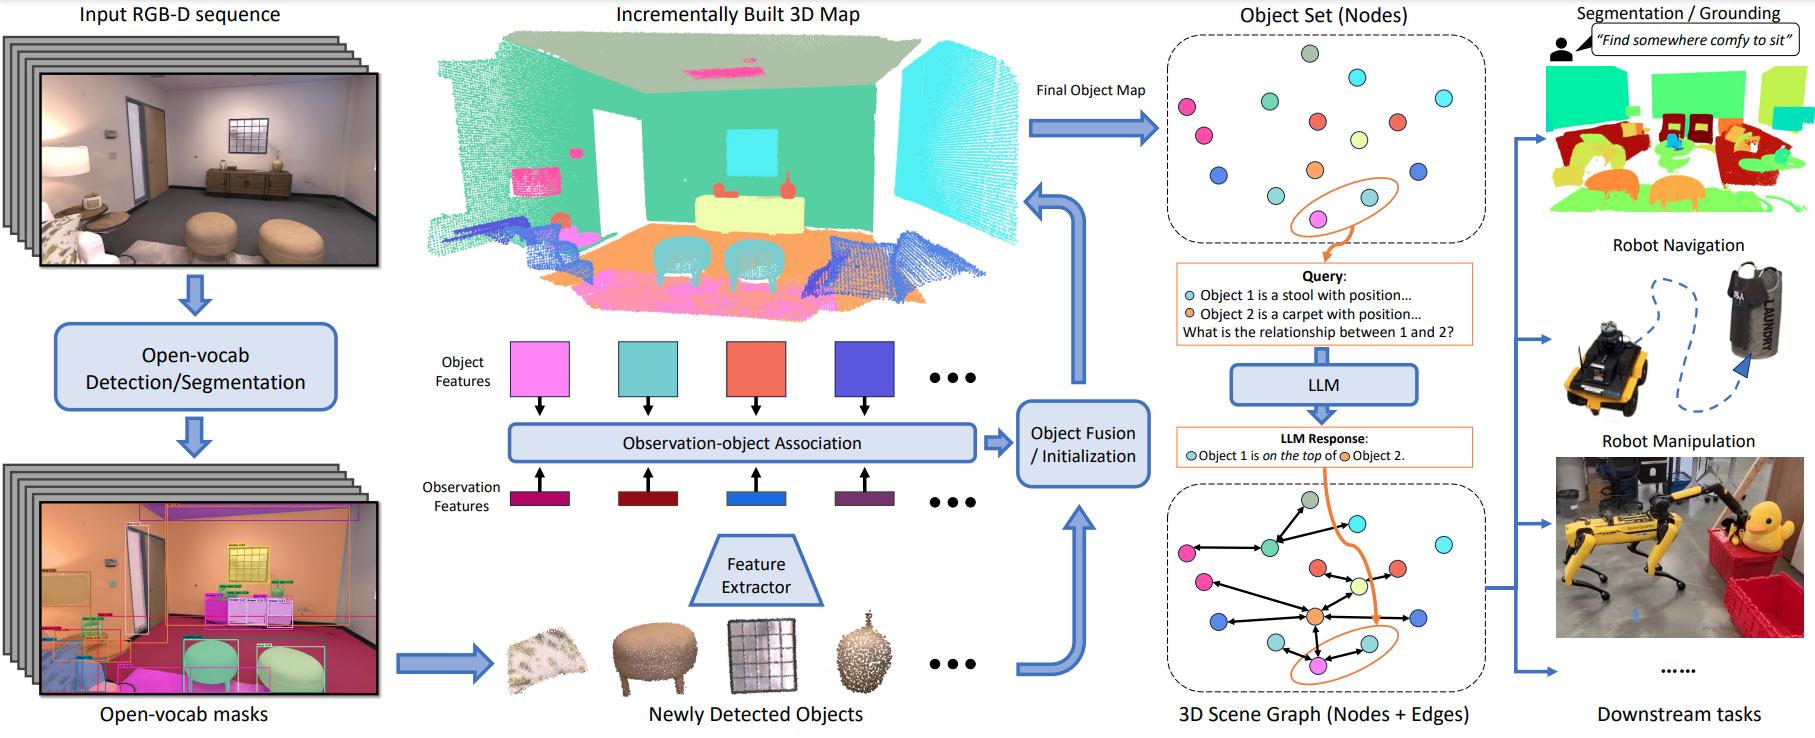
\includegraphics[width=0.8\linewidth]{images/concept-graphs-pipeline.png}
    \caption{\textbf{ConceptGraphs} is a framework for building sparse representations that are useful for Spatial AI. It process sequences of RGB-D images and builds a corresponding open vocabulary scene graph. This is achieved through class-agnostic object segmentation followed by querying a VLM model such as CLIP \cite{clip} to obtain an embedding. The relations between these entities in the graph are generated with an LLM.  See \url{https://concept-graphs.github.io/} for further details and videos. }
    \label{fig:concept-graph}
\end{figure}

This and similar methods (such as \cite{HOV-SG}) represent a breakthrough in that the types of queries that they can admit are substantially more general and abstract than previous closed-vocabulary methods. Furthermore, they enable  task specification to be conveyed through natural language, as opposed to previous methods which required, e.g., navigation coordinates in a world frame.

Nevertheless, these types of representations still has significant limitations, such as: 1) Object representations do not contain any information about affordances or ways in which an agent could interact with them; 2) The representation assumes that the world is static and that objects don't move; and 3) The representation is not conditioned on the specific skills that an agent is able to execute, and therefore can be of limited use for planning more complex tasks.


The main objective of this proposal is to overcome some of these limitations to progress towards \textbf{robotic agents that can seamlessly integrate into human environments and perform useful, complex, abstractly-specified tasks with sparse and intuitive supervision}.



%% -------------------------------
%% Partnership
%% -------------------------------
\section*{Partnership}
\ifinst\begin{instructions}
  \item List all partner organizations participating in the project. For each, describe their core activities and how they align with the project, their need for the proposed project, and their experience related to it, such as efforts to date to address the challenge.
  \item	Describe each partner organization's active role in the project, including defining the research questions, designing the research plan, collaborating or contributing to the research activities, co-supervising trainees and monitoring progress.
  \item Describe how the partner organizations will translate, mobilize and/or apply the research results to achieve the intended outcomes. 
  \item Explain the value and importance of each partner organization's involvement and other in-kind contributions to achieving the project's intended outcomes. If applicable, discuss how the combination of partner organizations is beneficial to the project. 
\end{instructions}\fi
  
Denso is the only partner organization expected to make contributions.

\textbf{describe their core activities and how they align with the project, their need for the proposed project, and their experience related to it, such as efforts to date to address the challenge.}

DENSO has been investing in AI for decades. The collaboration with the University of Montreal started in 2019.
DENSO has previously contributed a sum of 271K CAD in cash, and dispatched a senior employee to Montreal for a
year from 2019 to 2020, who was heavily involved in the algorithm development and problem definition.
For this proposal, DENSO will provide a direct cash contribution of 40000 CAD (this sum is over and
above the previous 364000 CAD which has been provided in previous years and is not eligible for
this proposal for a total of investment of  404000 CAD in the Montreal Robotics and Embodied AI Lab at the University of Montreal).

The Denso team comprises ....

The DENSO collaborators will take an active role in the research project, as they have since 2019. This includes monthly meetings where research progress and ideas are discussed. In between meetings there is a constant communication link through Microsoft Teams. The collaborators have been instrumental in defining and scoping the research problem. They have also run tests on their data and in their specific setup to validate the work that we are doing. Over the past five years, the Denso collaborators role in the research programme has been instrumental, including but not limited to: providing real world datasets, helping to analyse research results, providing feedback on research ideas, and helping to write research manuscripts. In short, they are active contributors to a very productive academic research collaboration.  

\todo{relate the concept graphs idea to advanced manufacturing}

Denso is planning to apply for patents as a result of the output of the work. 

%% -------------------------------
%% Proposal
%% -------------------------------
\section*{Research plan}
\ifinst\begin{instructions}
  \item Specify the research objectives and expected results. Describe the planned research activities, methodology and experimental design.
  \item Provide approximate timelines for the activities, milestones and deliverables. You may use a Gantt chart, table or diagram.
  \item Describe how equity, diversity and inclusion are considered in the research process (e.g., research questions, design, methodology, analysis, interpretation and dissemination of results) and how these considerations are integrated where relevant.
\end{instructions}\fi

We will address the limitations of existing methods listed above with the following objectives:

\begin{enumerate} [label=\textbf{[O\arabic*]}]
    \item Build a method for endowing entity (object) representations in the graph with  specific affordance or interaction information.  \label{L:affordance}
    \item  Develop a  representation faithfully represents dynamic and semi-static objects with a longer term objective of modeling how these objects tend to move in the environment over time.   \label{L:time}
    \item Build a simiulation-based workflow for robot-specific plan verification conditioned on the scene graph representation.  \label{L:grounded}
    
\end{enumerate}


Here we will detail the specific approaches that we take to achieve the objectes listed above. 

\textbf{Affordance-aware Representations (\ref{L:affordance}}):
% Sacha
Object-centric 3D scene graphs focus on object-level scene understanding. While sufficient to specify high-level navigation goals and simple manipulation objectives, more sophisticated tasks require interacting with specific object parts of objects such as handles, control knobs and switches.
We aim to augment the ConceptGraphs \cite{concept-graphs} representation with an interaction layer describing each interactive part in terms of (i) its geometry and (ii) its affordance, represented as the scene graph changes induced through interaction.
The result is a novel functional scene graph representation that maps perceptual inputs to a structure that directly supports complex task planning.
We also aim for our representation to support interactive perception.
Our goal is to predict initial affordances given the commonsense knowledge of vision-language models (VLMs) and refine them through experience, for example by discovering the effects of a specific switch via interaction and observation.


ConceptGraphs describes objects using open-vocabulary features and free-form language. We aim to do the same with interactive elements and avoid restricting our representation to a predetermined closed set of interactive parts. To this end, our scene graph inference pipeline integrates a number of foundation models to process incoming RGB-D data:
\begin{itemize}
    \item MASt3R~\cite{leroy2024grounding-mast3r} as part of the MASt3R-SLAM~\cite{murai2024mast3r-slam} system to obtain camera pose estimates from monocular RGB data.
    \item SAM~\cite{kirillov2023segment-SAM} to identify class-agnostic image segments.
    \item CLIP~\cite{clip} to extract segment-level semantic features.
    \item VLMs like Molmo~\cite{molmo2024} or Qwen2.5~\cite{bai2025qwen2} to ground specific object parts thanks to its pixel-pointing ability. We also use Molmo's more general language skills for task planning and querying tasks.
\end{itemize}

The outputs of all models are merged over time and combined in a global coordinate system to build a 3D functional representation that is ready for task planning. Crucially, we can leverage the fact that we are obtaining multiple views of objects to improve the affordance predictions as they should be consistent over time.

We will have a set of predifined affordances \footnote{future work will look into making this open vocabulary} that describe the type of operations our robot can perform on an object. 
We have already experimented with a simple model that takes the best view of each object stored in our ConceptGraph representation and asks it to find specific points that correspond to each of the considered affordances. These points are then fed as input to SAM to segment out the part of the image that can be interacted with. 
Three successful examples are shown in Fig.~/ref{fig:affordances}, but this approach has proven to be somewhat limited and needs further refinement, e.g., from incorporating multiple views of each object. 

\begin{figure}[h!]
    \centering
    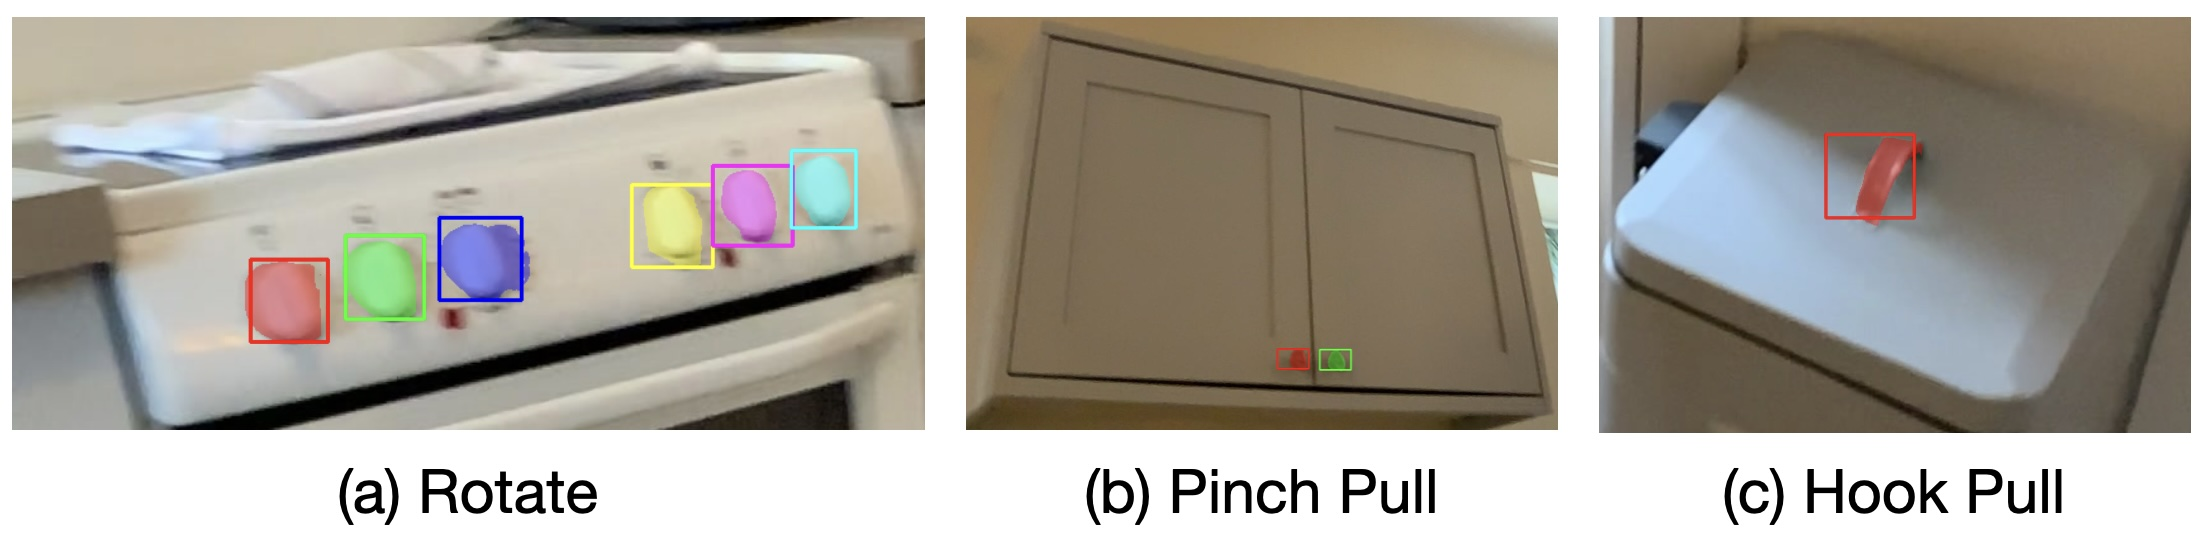
\includegraphics[width=0.8\linewidth]{images/affordances.jpg}
    \caption{Three examples of affordances correctly predicted and segmented by our model.}
    \label{fig:affordances}
\end{figure}

It is also noted that there is a newly published benchmarks SceneFun \cite{scenefun}, that has high quality point clouds generated from laser scans and is annotated with object affordances. This benchmark will be our initial quantitative evaluation of progress. 


\textbf{Time-varying Representations (\ref{L:time})}:
% Miguel + Francesco
%In the field of Spatial AI, the goal is to process the scene to establish a shared understanding of the environment for both human and robotic agents operating within it. Such scenes are inherently dynamic, since objects state (present or absent) and their position can change as a result of humans and/or robots interactions. However, modeling these world dynamics is a challenging task because it requires capturing the types of interactions external agents (e.g. humans) perform in the scene, such as the frequency and extent of their interactions with objects, as well as how object dynamics change due to these interactions. 
%
%Due to the nature of this complex modeling task, previous works have addressed only specific aspects rather than the problem as a whole. For example, Zhu \emph{et al.}~\cite{zhu2024living} studied how to reconstruct objects in 3D environments that undergo changes over time while simultaneously improving the registration of the point clouds of such objects. The downside of this approach is its purely geometric nature, with no exploration of strategies that could incorporate semantic priors to bypass some of the costly computations. On the other hand, Gorlo \emph{et al.} \cite{gorlo2024long} proposed a framework to study the dynamics of 3D scenes from the point-of-view of (expected) humans interaction by querying an LLM several times during training in order to fit their model and capture long-horizons (i.e. 60s) human trajectories in the scene. However, these results are based on the assumption that humans continuously interact with objects when they move in the scene, which is rarely true. 
%
%To address some of these limitations, i
In our recent work ``Perpetua''~\cite{saavedra2025perpetua} we take a first step towards understanding complex feature dynamics in semi-static environments (environments where elements change while we are not directly observing them). 
%In particular, Perpetua is capable of both modeling and \emph{predicting} whether a feature will be present or absent arbitrarily far into the future. Embedding map representations with predictive capabilities enhances their robustness to scene changes, even when those changes are not directly observed. Furthermore, predicting the future state of features (or objects) has also been useful for downstream tasks such as robot search for non-stationary objects \cite{krajnik2015waldo}. 
However, our approach has two main limitations: it assumes that a feature always appears and disappears in the same location, and it requires training a separate model for each feature in the map, making it difficult to scale to environments with thousands of features. To address these challenges and building on the success of world models in robotics applications~\cite{pi0, pmlr-v235-zhou24f}, our goal is to shift our paradigm to a centralized one in which we use a single world model to predict the spatio-temporal dynamics of \emph{all} features in the environment.

We aim to create a world model that captures the spatio-temporal dynamics of objects in the scene. The reasons we believe that this idea can be successfully addressed are numerous. First, objects do not move around in the environment following random patterns~\cite{schmid2022panoptic}; for example, you would expect to find forks and plates in the kitchen, but not in the bathroom. Furthermore, humans typically move objects according to predefined patterns: a remote control is likely to be moved back and forth between the table and the couch, but not placed on top of the washing machine. Additionally, when we are tasked to retrieve a particular object, we know beforehand which is the most likely place we can expect to find it. For instance, if someone cannot find their glasses or keys, they know where to check first to increase the chances of locating them.

These insights led us to explore a new strategy for \emph{commonsense-informed} and \emph{semantically-aware} task planning and object retrieval for robots in the world using semantic prior and LLMs. We call our approach \textbf{FlowMaps} since it employs Flow Matching \cite{lipman2022flow} to model a posterior distribution describing the position of objects in the scene after some time interval, \emph{because humans live in the world and move them around} in semantically coherent ways. Flow Matching models are computationally cheaper than Diffusion Models for generative applications \cite{lipman2022flow}, making them more suitable for use in robotics~\cite{pi0}. Nevertheless, training them to achieve a competitive performance is still computationally expensive and requires several hours of training on GPU-powered devices, plus a large amount of high-quality data.
 
%Lastly, we plan to deploy both robots simultaneously in collaborative task-planning scenarios to push the limits of our world model’s capabilities. 
 
\textbf{Simulation-in-the-loop (\ref{L:grounded})}: 
% Charlie
%
\newcommand{\todocite}[1]{{\textcolor{red}{(TODO CITE #1)}}}
%
%In the context of robotic planning, the ability of LLMs to store and retrieve the ineffable human understanding of the world shows great promise in enabling robots to perceive and plan over open-domain, open-vocabulary environments. By leveraging the semantic understanding and generative power of LLMs, it is possible to create robot plans for varying contexts and environments. 
%However, the knowledge retrieved from LLMs can also possess undesirable qualities, such as hallucinations \cite{10.1145/3571730}, lack of understanding of nuance and context \cite{10.1145/3442188.3445922}, and sycophancy \cite{sharma2024towards}. Bad actors can also \textit{jailbreak} LLMs \cite{wei2023jailbroken}, breaking the guidelines imposed upon them by their creators. Recent work has demonstrated that these issues can be exploited to support \textit{killer robots}: \cite{robey2024jailbreaking} showed that by telling an LLM that the robot it controls is part of an action movie, a bad actor can detonate bombs to harm humans. 
%
%The field of AI safety has exploded in recent years, but is mostly focused on the \textit{alignment problem}, which seeks make AI systems behave with human intentions and values \cite{ji2024aialignmentcomprehensivesurvey}. But, safety is not a novel concern in robotics whatsoever. Indeed, robotics has a long and storied history of \textit{safety by design}, with many checks and balances and safety measures to ensure robots operate as desired by their creators \cite{engelberger2012robotics}. However, the question of how best to apply these time-tested robotic design practices to embodied AI safety remains an open problem.
%
We plan to develop a \textit{plan verification} method for LLM-generated plans to enable LLM planners to be \textit{safe by design}. We do this by reconstructing the robot's environment in a realistic simulator (Isaac Sim) programmatically from its ConceptGraph \cite{concept-graphs} representation. Specifically, for each object, we compare their text embeddings (semantic latents) with the text embeddings of assets from the Objaverse \cite{objaverse} dataset of 3D assets using CLIP \cite{clip}. The LLM-generated plans are then rolled out in the reconstructed simulation, allowing us to ensure that each LLM-generation action obeys safety guidelines and that the final state of the simulation matches the desired final state defined by the task specification. This enables us to incorporate LLM-derived information such as the interactibility of objects into GPU-enabled physical and visual simulations.
%Another tool that can be useful in ensuring sane LLM-generated plans is the ability to provide them with feedback. In RoCo \cite{roco}, feedback was shown to significantly reduce plan failure rate.
Because of the ability of our proposed method to perform fine-grained plan verification, we also obtain a tool to provide feedback for LLM planners with detailed information about failure points or new skills that the robot should learn in order to be able to achieve its task. We then plan on learning or fine-tuning natural-language-guiding RL agents on these scenes built from real-world perception. This will enable fast real-to-sim-to-real loops for control through the use of NVIDIA GPUs.

%Our method is based on the ConceptGraph scene representation. We parse the list of objects in the scene, as well as geometric information (bounding box and position) and semantic information (LLM-generated descriptions). For each object, we compare their text embeddings (semantic latents) with the text embeddings of assets from Objaverse \cite{objaverse} (a large dataset of 3D assets) using CLIP \cite{clip}. This allows us to quickly obtain 3D assets without running into issues commonly associated with mesh-from-perception methods such as slow computation times and faulty object faces \cite{10.1007/978-3-031-59057-3_25}, etc. In a similar manner to Holodeck \cite{Yang_2024_CVPR} (based on AI2Thor \cite{ai2thor}), we then use the 3D assets to rebuild the real-world ConceptGraph as a simulated scene. This procedurally-generated simulator supports physics (picking up/placing down objects, moving objects, collisions, etc.) but does not support object-centric AI2Thor interactions such as OpenObject, BreakObject, etc. To enabled this facet, we task an LLM with generating labels for each object such as \texttt{isOpenable} and \texttt{isBreakable}, which we then parse as part of an additional \textit{semantic simulation layer}.

%We then use this scene reconstruction to roll out LLM-generated plans. We perform varied classical aspects of plan verification by using pre- and post-conditions. For instance, (1) to BreakObject an object, it must be ``isBreakable'', (2) after moving an object, we must update the geometric distance of each object in the scene representation (to enable (2), we must compute costly pairwise distances and verify pairwise volumetric overlaps; to render this tractable, we use the GPU-enabled \textit{Jax} framework \cite{jax2018github}). We also perform semantic plan verification by producing audits of the changes in the scene before and after using a robot skill, and providing LLMs with these audits as well as a prompt asking them to verify the safety and alignment of these changes. This enables us to prevent cases such as the killer robot dog we outline above. 

%The failure points of each plan can then be provided to the original LLM planner in order for it to change its plan, making LLM planning a closed-loop process, whereas most other LLM planning methods treat it as an open-loop process.

%\textit{Future work:} The method outline above is limited to LLM-generated plans. The robotics community uses the underlying AI2Thor simulator mostly for semantic planning, with physics simulation taking a less important role. After the publication of this method, we wish to apply the same idea to control instead of planning. This entails converting the JSON-described scenes generated from the ConceptGraph and Objaverse to the USD format intelligible by NVIDIA Omniverse \texttrademark. We then plan on learning or fine-tuning natural-language-guiding RL agents on these scenes built from real-world perception. This will enable fast real-to-sim-to-real loops for control through the use of NVIDIA GPUs.


%% -------------------------------
%% Team
%% -------------------------------
\section*{Team}
\ifinst\begin{instructions}
  \item List the applicant, any co-applicants, key participating staff of the partner organizations and any other key academic team members. For each, explain how their knowledge, expertise, experience and contributions align with the proposed project and describe their role in the project, as well as their roles and capabilities in training and mentoring trainees.
  \item	Briefly describe the plan for managing the project, along with the qualifications, roles and responsibilities of the team members involved in this respect.
\end{instructions}\fi
  

Liam Paull is an assistant professor at l'Université de Montréal and the co-founder of the Montreal
Robotics and Embodied AI Lab (REAL). His lab focuses on robotics problems including building
representations of the world (such as for simultaneous localization and mapping), modeling of
uncertainty, and building better workflows to teach robotic agents new tasks (such as through simulation
or demonstration). Previous to this, Liam was a research scientist at CSAIL MIT where he led the TRIfunded autonomous car project. He was also a postdoc in the marine robotics lab at MIT where he
worked on SLAM for underwater robots. He obtained his PhD from the University of New Brunswick in
2013 where he worked on robust and adaptive planning for underwater vehicles.

\todo{bio for Denso folks}

\todo{describe the rest of the research team}

%% -------------------------------
%% Training plan
%% -------------------------------
\section*{Training Plan}
\ifinst\begin{instructions}
  \item Describe the learning experiences the project will provide, including the nature of interactions between trainees (undergraduate and graduate students, postdoctoral fellows) and partner organizations. 
  \item	Describe the research and professional skills that trainees will develop through these experiences and through their roles in the project.
  \item Explain how the research and professional skills gained by the trainees will prepare them for their future careers.
  \item Describe challenges to equity, diversity and inclusion in the context of your project's training environment and specify concrete practices you will implement to address them. You are encouraged to cite evidence supporting the proposed practices and to describe how you will monitor and adapt your actions based on non-demographic indicators of success.
\end{instructions}\fi
  

In my research lab, I use  the following concrete practices to ensure that students are driven to achieve their potential while also maintaining a healthy work-life balance.
First, during mentorship it is understood that not all students will be amenable to the same types of guidance, feedback, and metrics of success.
All students will be given the opportunity, and in fact encouraged, to co-author conference papers and attend international conferences, present their work internally to the group and within the larger community, but none of these will be requirements for graduation or used as metrics for success.
Second, I allocate my students to small focused research groups and I meet with these groups on a weekly basis.
These meetings are primarily for discussing research and contain students at different stages of studies such that more senior students can gain mentorship skills.
I also meet with each student individually on a monthly basis to explicitly discuss non-research related issues such as career development and this is also a venue where any specific issues can be raised. This was a practice I started during the COVID-19 pandemic to ensure that students were coping, but have continued since it yielded so many benefits. 
Third, all students will be given the opportunity, and will be encouraged, to test algorithms using real-world datasets, and on hardware.
In so doing, each student has equal opportunity access to resources, including the robot hardware and supervision from their advisor.
Fourth, there is zero tolerance in the group and workplace for any type of harassment. Upon acceptance, students are presented with a document that outlines the specifics of this policy as well as what options and actions they can take in the event that they wish to report something.
%Fourth,  we  co-organize a weekly ``Robot Learning Seminar'' where we invite a diversity of speakers from a wide range of backgrounds investigating a wide range of topics, some technical, but others much more socio-technical.


I encourage my students to embrace social causes that do not directly impact their research portfolio. For example, one of my trainees contributed to the ``Declaration Montréal'' and to the UNESCO working groups on AI Ethics.
I also encourage my students to consider the broader implications of the work that they do. Robotics and automation has the potential to disproportionately affect certain demographics. In this sense I also try to lead by example, such as the Duckietown project whose core mission is the democratization of robotics, and by organizing and hosting workshops on this subject, such as the 2021 IROS workshop on ``Evaluating the Broader Impact of Self-driving Cars''. 



I believe wholeheartedly in the values of equity diversity and inclusion (EDI) and the tangible benefits that these principles bring. Above all else, I believe that everyone should be treated with kindness, respect, and equal opportunity, and it is my objective to lead my research group with these principles at the forefront.



Recruiting graduate students from diverse backgrounds is a challenge in computer science and robotics. The overwhelming majority of applications that I receive are from applicants that identify as male and originate from a select few countries. I recruit students primarily through the Mila admissions system or organically through the graduate and undergraduate courses that I teach. Mila has taken very significant and meaningful steps towards attracting and retaining students from underrepresented demographics, and whenever possible I leverage this in my own recruitment.
Nevertheless, I try to be aware of my own personal biases in the hopes to mitigate their effects. I have partaken in the Mila ``Leading for Equity and Inclusion'' workshop in 2022 where these concepts were central.


To date, I have successfully recruited three female graduate students and one female undergraduate student researcher.I have recruited one undergraduate student from Africa. Several of my graduate students are more mature and have started families, and I encourage them to manage their work-life balance appropriately. I am hoping to improve my recruitment from underrepresented demographics in the future by reaching out to specific groups that represent minorities in robotics, such as ``Queer in Robotics'', ``Black in Robotics'' and ``Women in Robotics''.  



Our research group has completed the ``Mila Community Sensitivity Workshop'', where we discussed specific notions related to EDI, including using inclusive language. 

In my research lab  the following concrete practices are employed to ensure training and development of students is equitable and inclusive.
First, during mentorship it is understood that not all students will be amenable to the same types of guidance, feedback, and metrics of success.
All students will be given the opportunity, and in fact encouraged, to co-author conference papers and attend international conferences, present their work internally to the group and within the larger community, but none of these will be requirements for graduation or used as metrics for success.
I allocate my students to small focused research groups and I meet with these groups on a weekly basis.
These meetings are primarily for discussing research.
I also meet with each student individually on a monthly basis to explicitly discuss non-research related issues such as career development and this is also a venue where any specific issues can be raised.
Second, all students will be given the opportunity, and will be encouraged, to test algorithms using real-world datasets, and on hardware.
In so doing, each student has equal opportunity access to resources, including the robot hardware and supervision from their advisor.
Third, there is zero tolerance in the group and workplace for any type of harassment. Upon acceptance, students are presented with a document that outlines the specifics of this policy as well as what options and actions they can take in the event that they wish to report something.
Fourth,  we  co-organize a weekly ``Robot Learning Seminar'' where we invite a diversity of speakers from a wide range of backgrounds investigating a wide range of topics, some technical, but others much more socio-technical.


I encourage my students to embrace social causes that do not directly impact their research portfolio. For example, one of my trainees contributed to the ``Declaration Montréal'' and to the UNESCO working groups on AI Ethics.
I also encourage my students to consider the broader implications of the work that they do. Robotics and automation has the potential to disproportionately affect certain demographics. In this sense I also try to lead by example, such as the Duckietown project whose core mission is the democratization of robotics, and by organizing and hosting workshops on this subject, such as the 2021 IROS workshop on ``evaluating the broader impact of self-driving cars'', as well as the ``AI Driving Olympics'' competitions which are designed to be accessible to anyone regardless of their background. As president of the Duckietown Foundation, we have donated robotics hardware to under-served communities in South America and Africa. 

The research agenda that I have outlined includes projects that range from fundamental to more applied. This is explicitly designed in order to appeal to a diversity of students. 


%% -------------------------------
%% Impact and benefits to Canada
%% -------------------------------
\section*{Impact and benefits to Canada}
\ifinst\begin{instructions}
  \item Explain how and the extent to which the proposed research will generate new knowledge in the natural sciences or engineering disciplines and/or develop or advance new technologies.
\item Considering the partner organizations' plans to use the research results, discuss how the project will lead to new or improved technologies, products, processes, services, policies, standards or regulations in Canada.
\item Describe how and the extent to which the project's intended outcomes will lead to economic, environmental, and/or other societal benefits to Canada and Canadians.
\end{instructions}\fi


I believe that the realization of my research vision has the potential to be transformative. My hope is that enabling robot technologies to operate in more complex and less structured environments allows their benefits to become accessible to all. To date we have seen robot technologies largely only in industrial settings where their core purpose is to increase manufacturing efficiency, which disproportionately benefits shareholders. However, robots operating in homes do not offset jobs and are potentially able to ease the burden of daily tasks for all. In short, I strongly believe in the democratizing  of this technology leading to social good, and this aligns well with Mila's core strategic priorities.

The specific Phase II objectives will have a significant impact on the field of robot learning, as they address several outstanding problems. We will demonstrate a pathway forward for robot representation learning that balances explicit structure and learning from data that is scalable yet efficient. This provides a backbone that could unlock other technologies. In particular, conditional scene generation  for robot skill learning could represent a paradigm shift in how we approach skill learning for robots. 


%% -------------------------------
%% References
%% -------------------------------
\newpage
\begingroup
\section*{References}
\renewcommand{\section}[2]{}%
\ifinst\begin{instructions}
  \item Use this section to provide a list of the most relevant literature references. Do not refer readers to websites for additional information on your proposal. Do not introduce hyperlinks in your list of references.
  \item These pages are not included in the page count.
\end{instructions}\fi
\bibliographystyle{abbrv}
\bibliography{udem-denso-alliance}
\endgroup

\end{document}
%% :wrap=soft:folding=explicit:
